\documentclass{article}
\usepackage{graphicx}
\usepackage{amsmath}
\usepackage[margin=2cm, top=2cm]{geometry}
\usepackage{tikz}
  \usetikzlibrary{angles, quotes}
  \usetikzlibrary{arrows.meta}
  \usetikzlibrary{positioning}
\usepackage{pgfplots}
  \pgfplotsset{compat=1.18}
\usepackage{amssymb}
\usepackage{enumitem}
\usepackage{tocloft}
  \renewcommand{\cftsecdotsep}{\cftdotsep}
  \cftpagenumbersoff{subsection}
\usepackage[normalem]{ulem}
\usepackage{dashundergaps}
\usepackage{xcolor}
\usepackage[most]{tcolorbox}

\definecolor{defmain}{HTML}{1d1280}
\definecolor{defbg}{HTML}{F4F8F7}
\definecolor{rpmain}{HTML}{790a73}
\definecolor{rpbg}{HTML}{F5F5F8}
\definecolor{zgmain}{HTML}{146609}
\definecolor{zgbg}{HTML}{F4F6F8}

\newtcolorbox{defbox}[2][]{
    enhanced,
    colback=defbg,
    colframe=defmain,
    arc=3mm,
    boxrule=0.6pt,
    leftrule=1mm,
    before upper={\textbf{\sffamily\color{defmain}#2}\par\vspace{8pt}},
    #1
}

\newtcolorbox{rpbox}[2][]{
    enhanced,
    colback=rpbg,
    colframe=rpmain,
    arc=3mm,
    boxrule=0.6pt,
    leftrule=1mm,
    before upper={\textbf{\sffamily\color{rpmain}#2}\par\vspace{8pt}},
    #1
}

\newtcolorbox{zgledbox}[2][]{
    enhanced,
    colback=zgbg,
    colframe=zgmain,
    arc=3mm,
    boxrule=0.6pt,
    leftrule=1mm,
    before upper={\textbf{\sffamily\color{zgmain}#2}\par\vspace{8pt}},
    #1
}

\newcommand{\babilon}{x_{n+1}=\dfrac{1}{2}\left( x_n + \dfrac{S}{x_n} \right)}

\title{Babilonska metoda}
\author{Gašper Mikložič}
\date{17.10.2026}

\begin{document}

\maketitle

\section{Formula}

\LARGE
$$x_{n+1}=\dfrac{1}{2}\left( x_n + \dfrac{S}{x_n} \right)$$
\normalsize

\section{Izvor in izpeljava}
Babilonska metoda izvira že iz starega Babilona, kjer so jo uporabljali za računanje kvadratnih korenov poljubnih števil in naj bi nastala med leti 1800 in 1600 pred našim štetjem.
Babilonci so jo verjetno izpeljali iz geometrije:
\begin{defbox}{Izpeljava}
\begin{center}
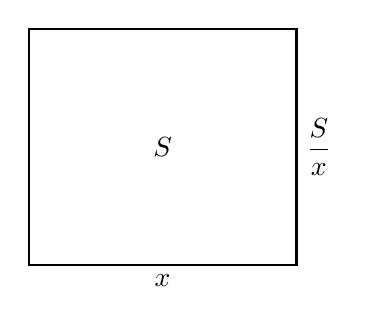
\begin{tikzpicture}
  \draw[thick] (0,0) rectangle (3.4,3);
  \node at (1.7,1.5) {$S$};
  \node[below] at (1.7,0) {$x$};
  \node[right] at (3.4,1.5) {$\dfrac{S}{x}$};
\end{tikzpicture}
\end{center}
Ko imamo pravokotnik s ploščino $S$ in je ena stranica $x$, je druga $\frac{S}{x}$.\\\\
Scimus:\\
\begin{itemize}
    \item $\frac{S}{x}\cdot x = S$
    \item Če je $x>\sqrt{S}$, potem je $\frac{S}{x}<\sqrt{S}$ in obratno
\end{itemize}
Zato lahko vzamemo aritmetično sredino teh dveh stranic in dobimo približno $\sqrt{S}$. To bi bil račun $\frac{1}{2}\left(x+\frac{S}{x}.\right)$\\
Potem si predstavljamo pravokotnik s stranico $x$ kjer je $x$ enak temu, kar smo dobili pri prejšnjem izračunu.\\
To ponavljamo, dokler dvakrat ne dobimo iste rešitve ali nismo zadovoljni z odgovorom.
\end{defbox}


\end{document}